\documentclass{article}
\usepackage[a4paper, total={7.5in, 10.5in}]{geometry}
\usepackage{graphicx}
\usepackage[export]{adjustbox}
\usepackage{xcolor}
\usepackage{array}
\usepackage{wrapfig}
\usepackage{lipsum}
\usepackage{ragged2e}
\usepackage[english]{babel}

\renewcommand{\baselinestretch}{0.95}
\setlength{\arrayrulewidth}{0.3mm}
\setlength{\tabcolsep}{5pt}
\renewcommand{\arraystretch}{1.7}
\begin{document}
	\begin{wrapfigure}{r}{2cm}
	\begin{center}
		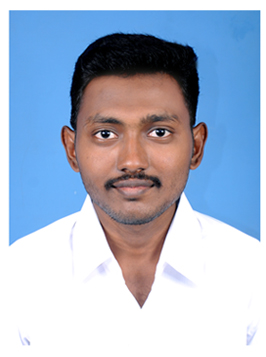
\includegraphics[width=47pt]{Infantraj}
	\end{center}	
	\end{wrapfigure}
	\huge \textbf{\\INFANT RAJ F}  \\
	\large 374/1, AssisiNagar, Sanyasigundu Extn.,\\
	Kitchipalayam(P.O), Salem - 636015, TamilNadu, India.\\
	Email ID: infantfdr@gmail.com Phone No.:+91 8438383635\\
	\hrule 
	\large \textbf{\\Career Objective}\\
	\hspace*{20pt} To work in a challenging environment where I can contribute my talents and skills for the optimum growth and development of the organization.
	\large \textbf{\\Education}
	\begin{table}[h!]
		\begin{center}
			\begin{tabular}{| m{3cm} | m{10cm} | m{1.5cm} | m{3.6cm} |}
				\hline
				\large\centering\textbf{Course} & \large\centering\textbf{Institution} &  \large\centering\textbf{Year} & \large\hspace{6pt}\textbf{Performance}\\
				\hline
				\large\centering B.E. (EEE) & \large\centering Knowledge Institute of Technology, Salem & \large\centering 2020 & \large\hspace{10pt} 6.62* (CGPA)\\
				\hline
				\large\centering HSC & \large\centering St.John's Matric. Hr. Sec. School, Salem & \large\centering 2016 & \large\hspace{30pt}76.67\% \\
				\hline
				\large\centering SSLC & \large\centering St.Thomas Matriculation School, Salem & \large\centering 2014 & \large\hspace{30pt} 89.20\%\\
				\hline
				\multicolumn{4}{c}{\color{white}right}
				{\large*upto 6\textsuperscript{th} Semester} 
			\end{tabular} \end{center} \end{table} \hfill 
	\begin{flushleft}
		\large \textbf{Projects}
		\begin{enumerate}
				\setlength\itemsep{0.01em}
			\item Agribot 1.0
			\item Smart Home IoT
			\item Analog Line Follower Robot
			\item Temperature Controlled Automatic Fan Regulator
			\item Car Accident Prevention System
		\end{enumerate}
		\large \textbf{\\* Training and Internship}\
		\begin{itemize}
			\setlength\itemsep{0.01em}
			\item Underwent One week Inplant Traning on \textbf{Electrical Control Unit} at \textbf{JSW Pvt. Ltd.,} Salem in 2018.
			\item Underwent One week Training on \textbf{PLC and SCADA} organized by \textbf{Center of Excellence for Industrial Automation (Powered by SIEMENS)} as a part of Value Added Course in 2017. 
			\item Underwent One week Inplant Training on \textbf{Electrical Maintainance} at \textbf{Steel Authority of India Limited,} Salem in 2017.
			\item Underwent One week Inplant Training on \textbf{Embedded Systems} at \textbf{Sans Innovation}, Salem in 2017. 
		\end{itemize}
		\large \textbf{\\Technical Skills}\
		\begin{itemize}
				\setlength\itemsep{0.01em}
			\item \textbf{Core Skills	:} AC to DC Converters,	Robotics and Automation using Atmega 328p Microcontroller, IOT using NodeMCU
			\item \textbf{Programming Languages	:}	C, C++ (Basic Level)
			\item \textbf{Software Tools	:}	MATLAB, Proteus, Circuit MOD, TeXstudio, MS(Word, PowerPoint, Excel)
			\item \textbf{Other Skills	:} Photoshop, Cyberlink Powerdirector
		\end{itemize}
		\large \textbf{\\Soft Skills}\
		\begin{enumerate}
				\setlength\itemsep{0.01em}
			\item Teamwork
			\item Time Management
			\item Flexibility
			\item Design sense
			\item Attentive and Self-monitoring
			\item Listening
		\end{enumerate}
		\large \textbf{\\Extra Curricular Activities}
		\item \textbf{Clubs and Forums}
			\begin{itemize}
					\setlength\itemsep{0.01em}
				\item Student Member in MHRD-IIC since Jan 2019.	
				\item Member in Rotaract Club at KIOT.
				\item Member in Instrumentation and Control Engineers Club at KIOT.
				\item Member in Indian Society for Technical Education (ISTE).
			\end{itemize}
		\large \textbf{\\Co-Curricular Activities}
		\begin{itemize}
			\item \textbf{Contests and Presentations}
			\begin{enumerate}
					\setlength\itemsep{0.01em}
				\item Received \textbf{"Judges Choice Category Award"} for the project titled \textbf{Agribot 1.0} in National Finals of e-Yantra Ideas Competition 2019 conducted by IIT Bombay.  
				\item Won \textbf{Third Prize} in Paper Presentation titled on \textbf{Smart Home IoT} in EDISON 2K18, A National Level Technical Symposium at Sona College of Technology, Salem in 2018.
				\item Won \textbf{Third Prize} in Paper Presentation titled on \textbf{Temperature Controlled Automatic Fan Regulator} in SYNERGY 2K18, A National Level Technical Symposium at Government College of Engineering, Salem in 2018.
				\item Won \textbf{Second Prize} in Make a Product Expo titled on \textbf{Temperature Controlled Automatic Fan Regulator} conducted by AMBERZ’ association, Knowledge Institute of Technology, Salem in 2018.
			\end{enumerate}
			\item \textbf{Workshops and Seminars}
			\begin{enumerate}
					\setlength\itemsep{0.01em}
				\item Participated a Seminar on \textbf{Recent Technologies in Autonomous and Hybrid Vechicles} by IEEE at Knowledge Institute of Technology, Salem in 2019.
				\item Attended One Day Workshop titled on \textbf{PLC and SCADA} conducted at Karpagam College of Engineering, Coimbatore in 2018.
				\item Attended One Day Workshop titled on \textbf{IOT using Arduino Nano and ESP8266} conducted by Top Engineers at IIT Madras in 2018.
				\item Attended One Day Workshop titled on \textbf{Robotics} conducted by Master Technologies, Salem in 2018.
			\end{enumerate}
		\end{itemize}	
		\large \textbf{\\Personal Details}
		\begin{table}[h]
				\begin{tabular}{m{2.8cm} m{0.15cm} m{3cm} }
				\large Father's Name & \large : & \large Francis D\\ 
				\large Mother's Name & \large : & \large Lourdumary F\\
				\large Date of Birth & \large : & \large June 29, 1998\\
		\end{tabular} \end{table}\\
		\large \textbf{\\Date : }
		\large \textbf{\\Place:  }	\hspace{360pt}\textbf{INFANT RAJ F}
	\end{flushleft}
\end{document}